\documentclass{article}
\usepackage{graphicx}
\usepackage{float}
\usepackage[utf8]{inputenc}
	itle{Examen 2: Motor Molecular Flashing Ratchet}
uthor{Grupo 2}
egin{document}
\maketitle
\section{Introduccion}
Este documento presenta la simulacion de un Flashing Ratchet implementado en C++.
\section{Resultados}
A continuacion se presentan las graficas obtenidas de la simulacion.
egin{figure}[H]
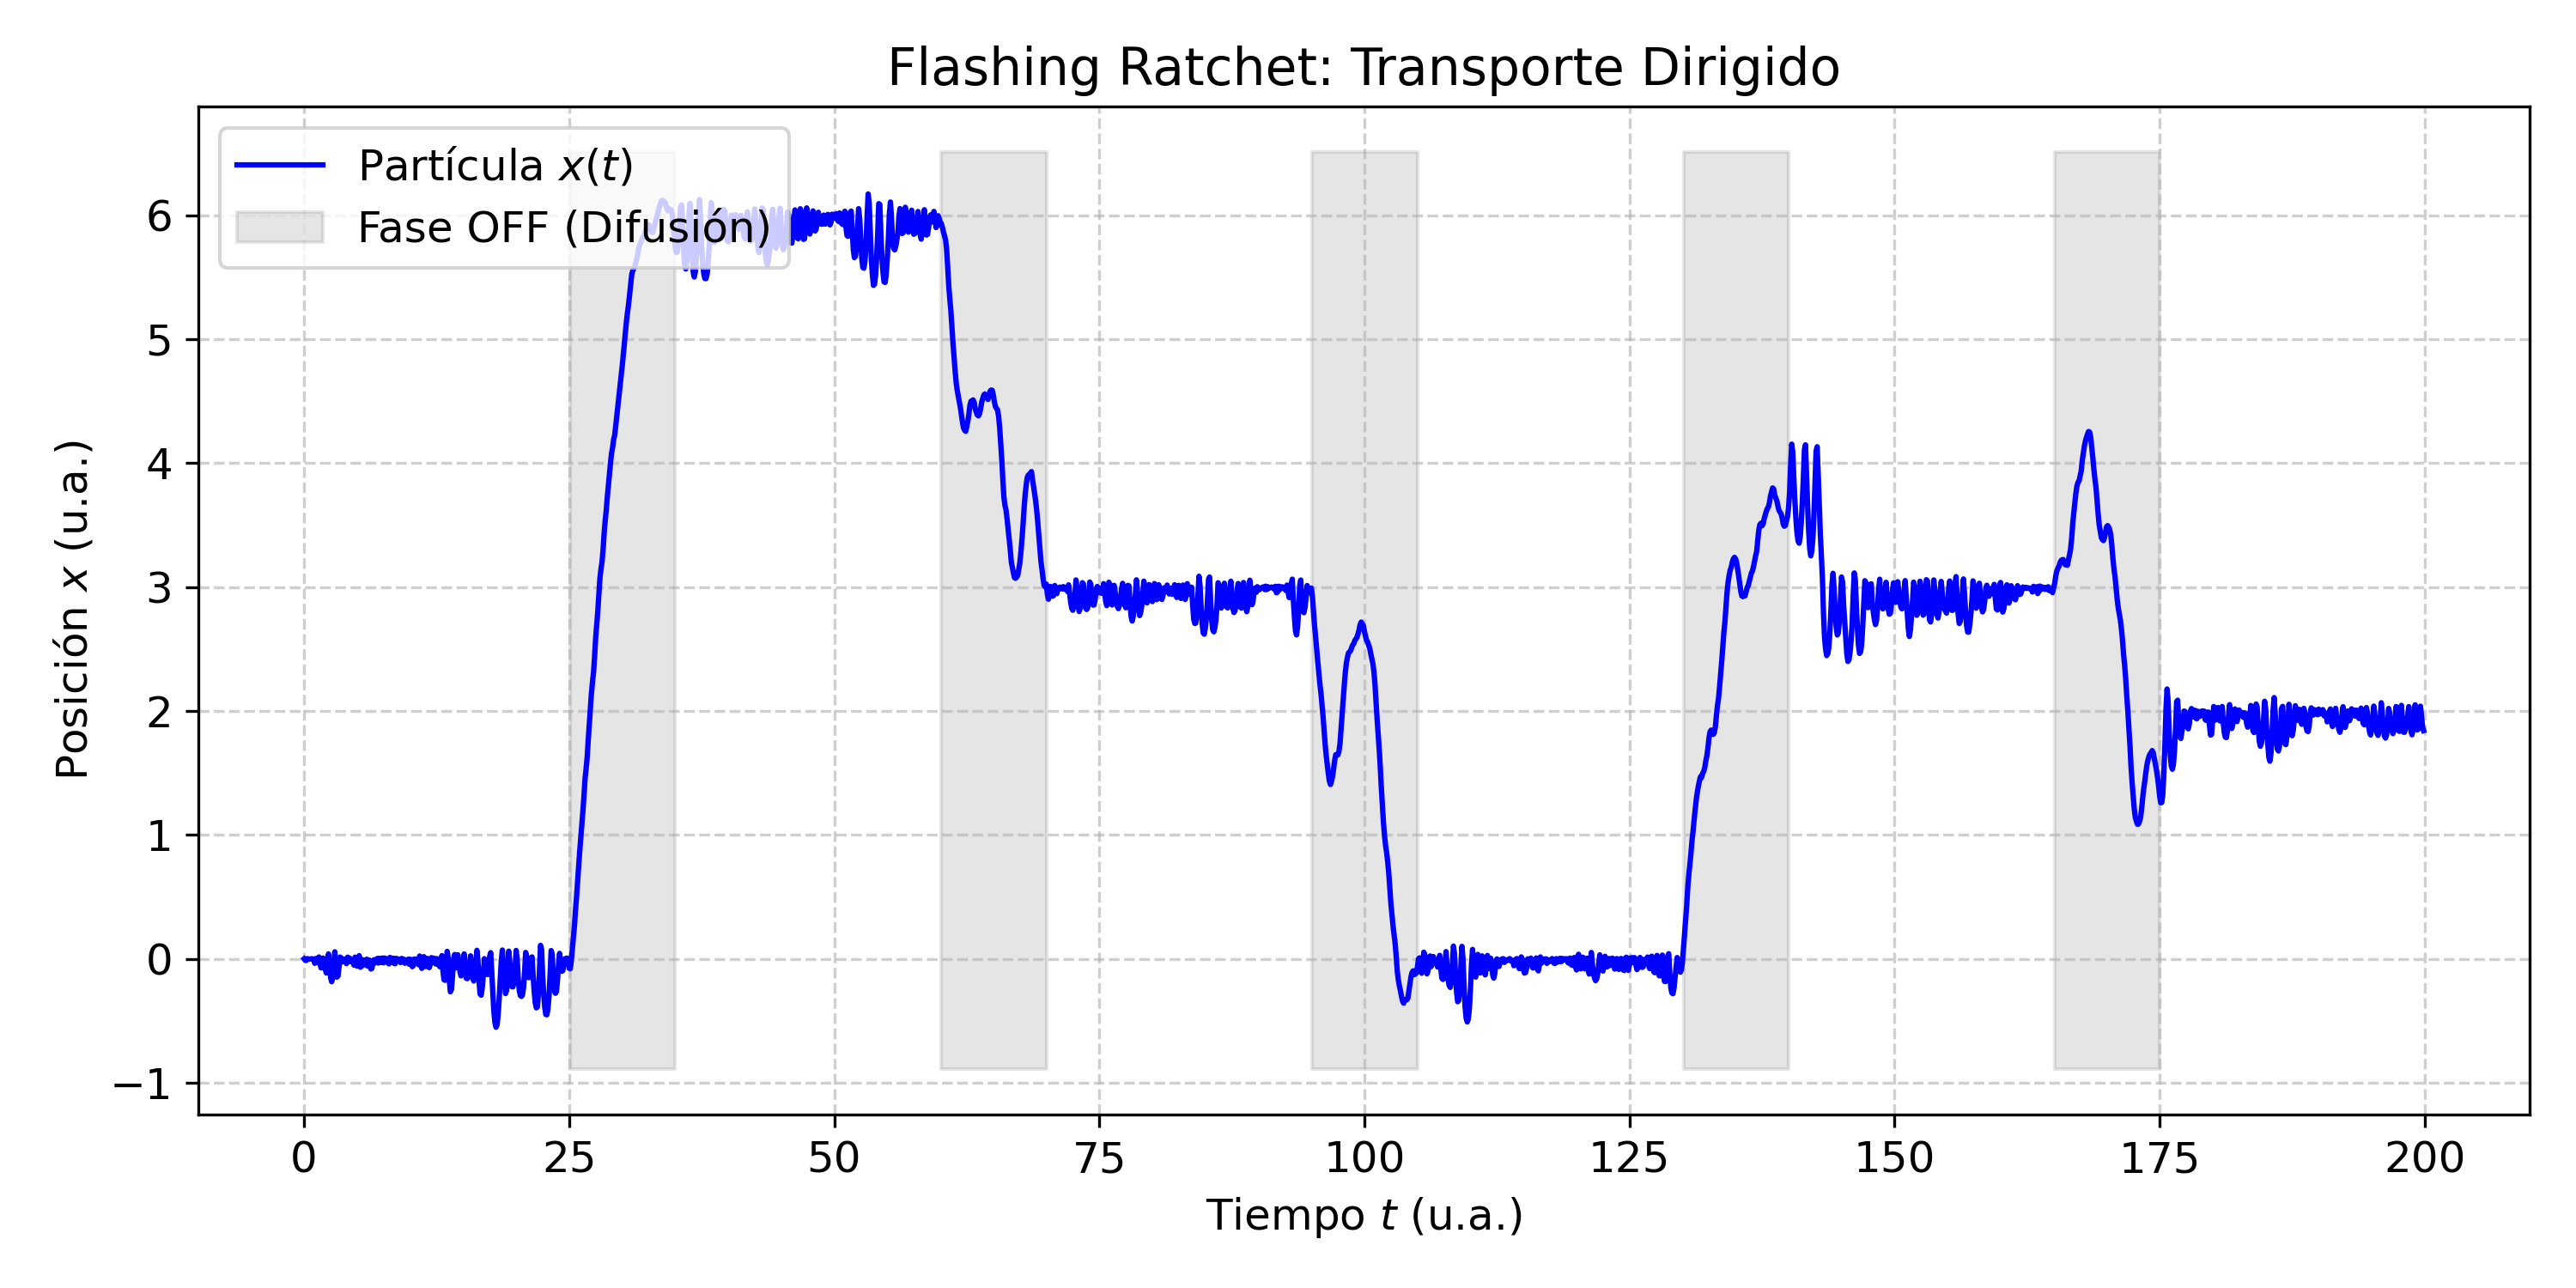
\includegraphics[width=0.9	extwidth]{../results/trayectoria.png}
nd{figure}
egin{figure}[H]

\includegraphics[width=0.9	extwidth]{../results/energia.png}
nd{figure}
egin{figure}[H]
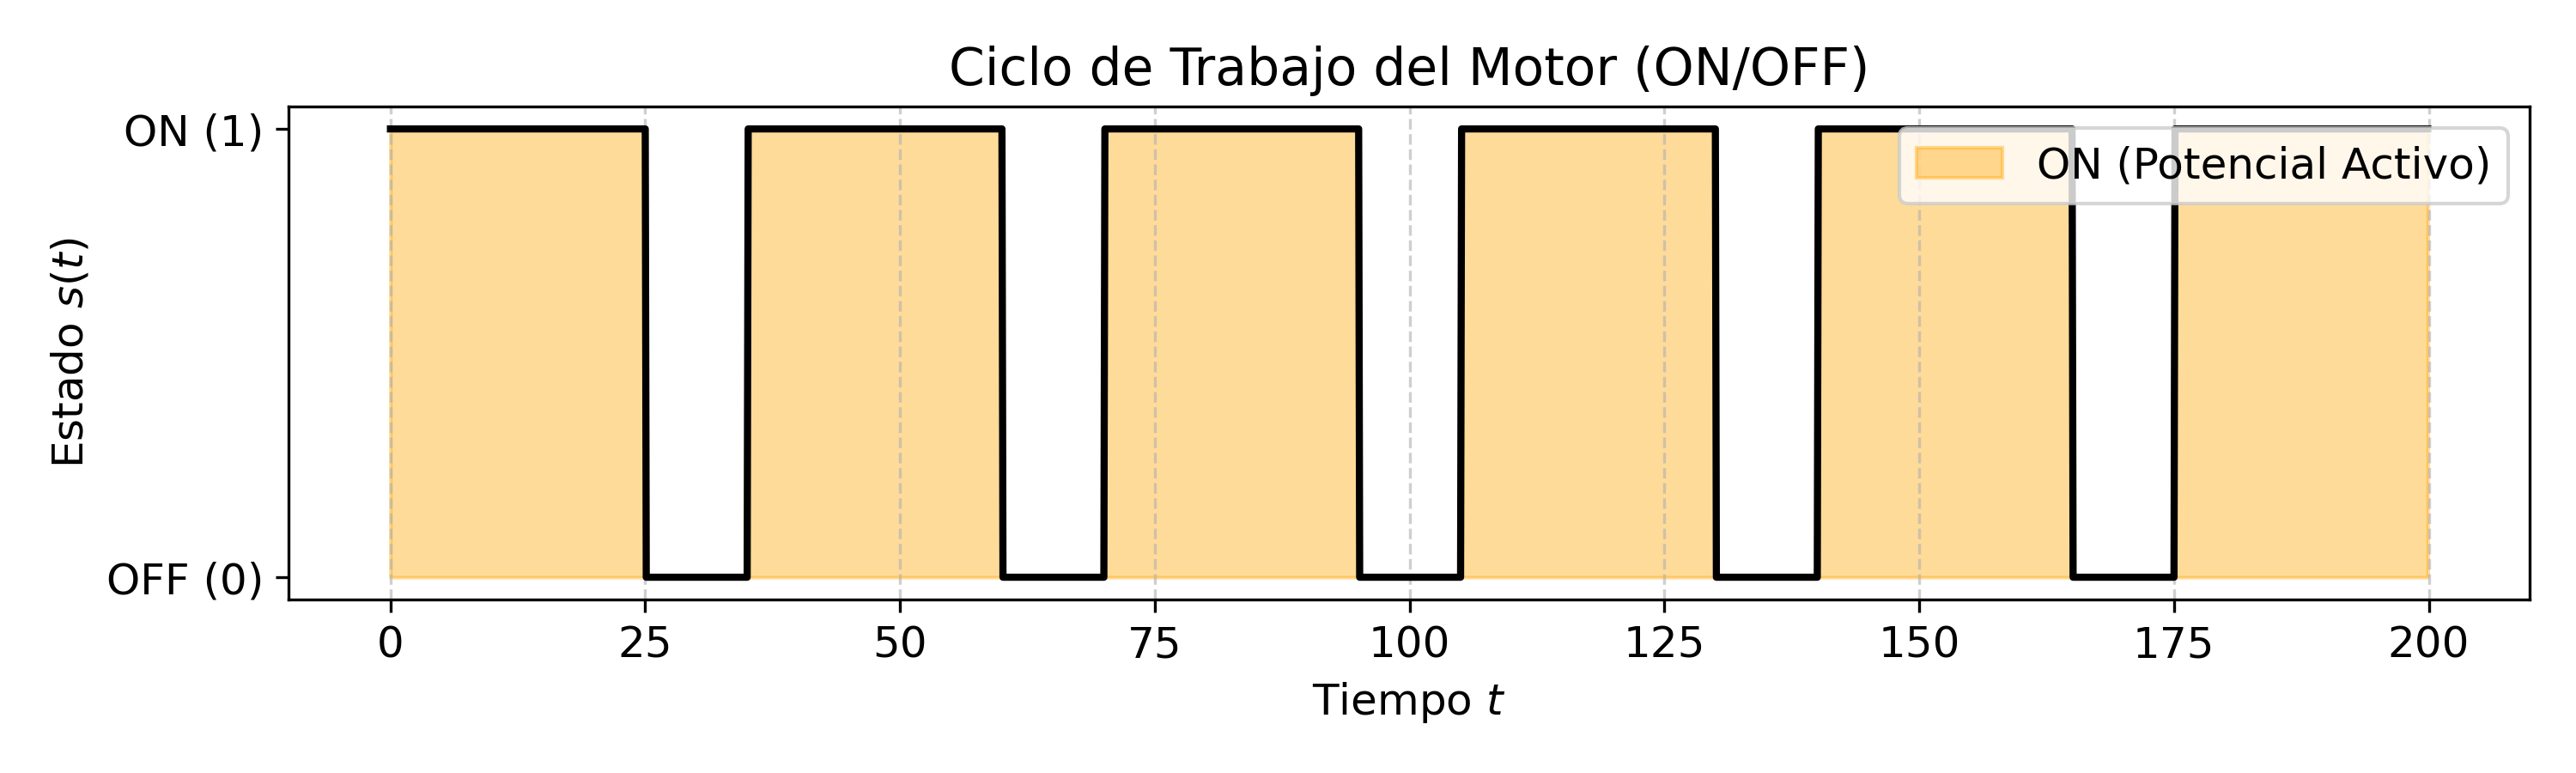
\includegraphics[width=0.9	extwidth]{../results/estados.png}
nd{figure}
nd{document}
